\documentclass[12pt, answers]{exam}
\usepackage[utf8]{inputenc}

\usepackage[margin=1in]{geometry}
\usepackage{amsmath,amssymb}
\usepackage{multicol}
\usepackage[]{graphicx}
\usepackage[]{bm}
\usepackage[]{nicefrac}
\usepackage[]{xcolor}

\newcommand{\class}{Physique non-linéaire}
\newcommand{\term}{Master 2}
\newcommand{\examnum}{Examen final -- Correction}
\newcommand{\examdate}{Février 2019}

\pagestyle{head}
\firstpageheader{}{}{}
\runningheader{\class}{\examnum\ - Page \thepage\ of \numpages}{\examdate}
\runningheadrule

\begin{document}

\noindent
\begin{tabular*}{\textwidth}{l @{\extracolsep{\fill}} r @{\extracolsep{6pt}} l}
  \textbf{\examnum} &&\\
  \textbf{\examdate} &&\\
\end{tabular*}\\
\rule[2ex]{\textwidth}{2pt}

Ce sujet contient \numpages\ pages (en comptant la page de garde) et \numquestions\ exercices.\\
Le nombre total de point est de \numpoints.

\begin{center}
  Barême\\
  \bigskip
  \addpoints
  \gradetable[v][questions]
\end{center}

\noindent
\rule[2ex]{\textwidth}{2pt}

\begin{questions}

\question[10] \textbf{Système de fonctions itérées: la courbe de Koch}
  \noaddpoints

  \begin{figure}
    \centering
    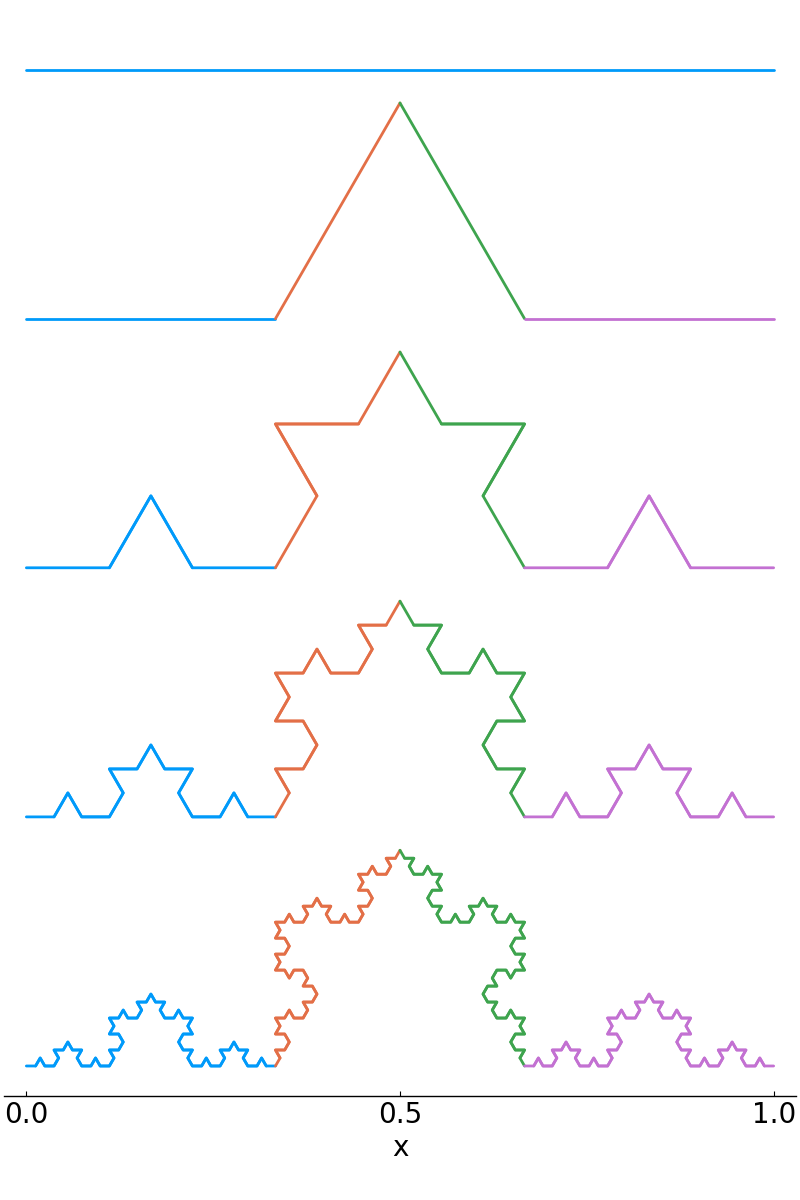
\includegraphics[height=.6\textheight]{imgs/koch_curve.png}
    \caption{Premières étapes de la construction de la courbe de Koch. \`A titre indicatif, chacun des angles d'un triangle equilatéral vaut 60$^\circ$.}
    \label{fig: koch curve}
  \end{figure}

  La construction de la courbe de Koch est décrite schématiquement sur la figure \ref{fig: koch curve} (voir page suivante). On cherche dans cet exercice à décrire cette construction à l'aide d'un système de fonctions itérées.

  \begin{parts}
    % -----> Points fixes et stabilité linéaire.
    \part[3] Donnez l'expression des quatres transformations affines $\bm{f}_i(\bm{x}) = \bm{A}_i \bm{x} + \bm{b}_i$ permettant de construire cette courbe avec $\bm{x} = (x, y)$. Expliquez en quoi consiste chacune des ces quatres transformations.

    \begin{solution}
      {\color{blue}
      Les quatres transformations affines recherchées sont les suivantes :
      \begin{equation}
        \begin{aligned}
          \bm{f}_1(x, y)  & = \begin{bmatrix}
                                \nicefrac{1}{3} & 0 \\
                                0 & \nicefrac{1}{3}
                              \end{bmatrix}
                              \begin{bmatrix}
                                x \\ y
                              \end{bmatrix} \\
          \bm{f}_2(x, y)  & = \begin{bmatrix}
                                \nicefrac{1}{6} & \nicefrac{-\sqrt{3}}{6} \\
                                \nicefrac{\sqrt{3}}{6} & \nicefrac{1}{6}
                              \end{bmatrix}
                              \begin{bmatrix}
                                x \\ y
                              \end{bmatrix}
                              +
                              \begin{bmatrix}
                                \nicefrac{1}{3} \\ 0
                              \end{bmatrix} \\
          \bm{f}_3(x, y)  & = \begin{bmatrix}
                                \nicefrac{1}{6} & \nicefrac{\sqrt{3}}{6} \\
                                \nicefrac{-\sqrt{3}}{6} & \nicefrac{1}{6}
                              \end{bmatrix}
                              \begin{bmatrix}
                                x \\ y
                              \end{bmatrix}
                              +
                              \begin{bmatrix}
                                \nicefrac{1}{2} \\ \nicefrac{\sqrt{3}}{6}
                              \end{bmatrix}\\
          \bm{f}_4(x, y)  & = \begin{bmatrix}
                                \nicefrac{1}{3} & 0 \\
                                0 & \nicefrac{1}{3}
                              \end{bmatrix}
                              \begin{bmatrix}
                                x \\ y
                              \end{bmatrix}
                              +
                              \begin{bmatrix}
                                \nicefrac{2}{3} \\ 0
                              \end{bmatrix}.
        \end{aligned}
      \end{equation}
      En rapport à la figure \ref{fig: koch curve}, chacune de ces transformations affines permet d'obtenir l'un des segments de couleurs ($\bm{f}_1 \to$ bleu, $\bm{f}_2 \to$ orange, $\bm{f}_3 \to$ vert et $\bm{f}_4 \to$ violet).
      }
    \end{solution}

    \part[2] Montrez que chacune de ces transformations est contractante (i.e.\ les valeurs propres de chacune des matrices $\bm{A}_i$ sont comprises dans le cercle unité).

    \begin{solution}
      {\color{blue}
      Pour chacune des matrices intervenant dans les différentes transformations affines décrites à la question précédente, le module des valeurs propres est à chaque fois
      %
      $$
      \vert \lambda \vert = \nicefrac{1}{3} < 1.
      $$
      %
      Par conséquent, ces quatres transformations $\bm{f}_i(x, y)$ sont toutes contractantes.
      }
    \end{solution}

    \part[2] La courbe de Koch est la courbe limite obtenue en appliquant les transformations affines $\bm{f}_i(\bm{x})$ un nombre infini de fois. Démontrez que sa longueur est infinie.

    \begin{solution}
      {\color{blue}
      Soit $L_k$ la longueur d'un segment et $N_k$ le nombre de segments composant la figure à l'itération $k$. Le longueur totale de la courbe à l'itération $k$ est alors $P_k = N_k \times L_k$. On a :
      %
      \begin{itemize}
        \item Itération 0 : $L_0 = 1$, $N_0 = 1$ et donc $P_0 = 1$.

        \item Itération 1 : $L_1 = \nicefrac{1}{3}$, $N_1 = 4$ et donc $P_1 = \nicefrac{4}{3}$.

        \item Itération 2 : $L_2 = \nicefrac{1}{3^2}$, $N_2 = 4^2$ et donc $P_2 = \left( \nicefrac{4}{3} \right)^2$.

        \item $\cdots$

        \item Itération $k$ : $L_k = \nicefrac{1}{3^k}$, $N_k = 4^k$ et donc $P_k = \left( \nicefrac{4}{3} \right)^k$.
      \end{itemize}
      %
      De là, il est facile de montrer que
      $$
      \lim_{k \to +\infty} P_k = +\infty.
      $$
      }
    \end{solution}

    \part[3] Quelle est la dimension fractale de cet objet?

    \begin{solution}
      {\color{blue}
      La dimension fractale de la courbe de Koch est
      $$
      D = \displaystyle \frac{\log(4)}{\log(3)}.
      $$
      }
    \end{solution}

  \end{parts}
  \addpoints

\bigskip
\question[10] \textbf{Réduction sur la variété centrale: le système de Lorenz}
  \noaddpoints

  Considérons le système de Lorenz donné par
  \begin{equation}
    \left\{
    \begin{aligned}
      & \dot{x} = \sigma \left( y - x \right) \\
      & \dot{y} = x \left( \rho - z \right) - y \\
      & \dot{z} = - \beta z + xy.
    \end{aligned}
    \right.
    \label{eq: lorenz system}
  \end{equation}
  Dans la suite de cette exercice, on supposera que les paramètres $\sigma > 0$ et $\beta > 0$ sont fixés. L'objectif de cet exercice est de caractériser la première bifurcation rencontrée par le système.

  \medskip

  \begin{parts}
    \part On s'intéresse dans un premier temps à la stabilité du point fixe
      $$
      (x^*, y^*, z^*) = (0, 0, 0)
      $$
      pour $0 \le \rho < 1$. Pour cela, introduisons la fonction potentielle donnée par
      $$
      V(x, y, z, t) = \displaystyle \frac{x(t)^2}{\sigma} + y(t)^2 + z(t)^2 \ge 0.
      $$
      \begin{subparts}
        \subpart[2] Montrez que l'équation différentielle gouvernant la dynamique de $V$ peut être mise sous la forme suivante
        $$
        \displaystyle \frac{\mathrm{d}V}{\mathrm{d}t} = -2 \left( x - \frac{1+\rho}{2}y \right)^2 - 2 \left( 1 - \frac{(1+\rho)^2}{4} \right) y^2 - 2 \beta z^2.
        $$

        \begin{solution}
          {\color{blue}
          En partant de l'expression de la fonction potentielle $V$, on peut écrire
          %
          $$
          \displaystyle \frac{\mathrm{d} V}{\mathrm{d}t} = \displaystyle \frac{1}{\sigma} \frac{\mathrm{d}}{\mathrm{d}t}x^2(t) + \frac{\mathrm{d}}{\mathrm{d}t}y^2(t) + \frac{\mathrm{d}}{\mathrm{d}t}z^2(t).
          $$
          Cette équation peut également s'écrire sous la forme
          %
          $$
          \displaystyle \frac{\mathrm{d} V}{\mathrm{d}t} = \displaystyle \frac{2 x(t) \dot{x}(t)}{\sigma} + 2y(t)\dot{y}(t) + 2z(t)\dot{z}(t).
          $$
          %
          En insérant dans l'équation ci-dessus l'expression de $\dot{x}$, $\dot{y}$ et $\dot{z}$, puis en regroupant les différents terms, on retrouve alors l'équation demandée.
          }
        \end{solution}

        \subpart[2] Montrez que, pour $0 \le \rho < 1$, cette fonction potentielle est strictement décroissante au cours du temps.

        \begin{solution}
          {\color{blue}
          On cherche à montrer que $\nicefrac{\mathrm{d}V}{\mathrm{d}t} \leq 0 \ \forall t$. En partant de l'expression obtenue à l'équation précédente, il est facilement de montrer que $V(t)$ est strictement décroissante au cours du temps si
          %
          $$
          1 - \frac{(1 + \rho)^2}{4} \geq 0.
          $$
          %
          On peut alors écrire
          %
          $$
          \begin{aligned}
            1 & > \displaystyle \frac{(1 + \rho)^2}{4} \\
            4 & > ( 1 + \rho )^2 \\
            2 & > 1 + \rho > -2 \\
            1 & > \rho > -1.
          \end{aligned}
          $$
          %
          Par conséquent, pour $0 \leq \rho < 1$, la fonction potentielle $V(t)$ est bien strictement décroissante au cours du temps.
          }
        \end{solution}

        \subpart[1] En conclure quant à la stabilité du point fixe $(x^*, y^*, z^*) = (0, 0, 0)$. Existe-t'il d'autres attracteurs pour $0 \le \rho < 1$?

        \begin{solution}
          {\color{blue}
          Posons $\hat{x} = \nicefrac{x}{\sqrt{\sigma}}$. La fonction $V(t)$ peut alors se ré-écrire sous la forme $V(t) = \hat{x}^2(t) + y^2(t) + z^2(t)$. Pour une condition initiale donnée $\bm{x}(0)$, cette fonction potentielle décrit donc l'évolution au cours du temps d'une forme de distance (au carré) de $\bm{x}(t)$ par rapport à l'origine de l'espace des phases. $V(t)$ étant une fonction strictement décroissante au cours du temps, on a alors que toute condition initiale est inévitablement attirée vers l'origine. Le point fixe $(x^*, y^*, z^*) = (0, 0, 0)$ est donc non seulement stable mais il est également le seul point fixe existant pour $0 \leq \rho < 1$.
          }
        \end{solution}

      \end{subparts}

    \part On cherche maintenant à caractériser le type de bifurcation ayant lieu pour $\rho_c = 1$. Pour cela, l'analyse se fera en deux temps.

    \begin{subparts}
      \subpart[1] Donnez l'expression de la matrice Jacobienne $\bm{J}$ du système linéarisé autour du point fixe $(x^*, y^*, z^*) = (0, 0, 0)$ et montrez que, pour $\rho = 1$, ses valeurs propres sont données par
      $$
      \lambda_1 = 0, \ \lambda_2 = -(\sigma + 1), \ \text{et } \lambda_3 = -\beta.
      $$

      \begin{solution}
        {\color{blue}
        Pour $\rho = 1$, la matrice Jacobienne du système de Lorenz linéarisé autour du point fixe $(x^*, y^*, z^*) = (0, 0, 0)$ est donnée par
        %
        $$
        \bm{J} = \begin{bmatrix}
                  -\sigma & \sigma & 0 \\
                  1 & -1 & 0 \\
                  0 & 0 & -\beta
                \end{bmatrix}.
        $$
        %
        Cette matrice étant diagonale par bloc, il est facile de montrer que ses valeurs propres sont effet données par
        %
        $$
        \lambda_1 = 0, \ \lambda_2 = -(\sigma + 1), \ \text{et } \lambda_3 = -\beta.
        $$
        }
      \end{solution}

      \subpart[3] Afin de déterminer le type de bifurcation rencontrée, faisons le changement de variable $r = \rho - 1$ de sorte à ce que l'équation pour $y$ s'écrive
      $$
      \dot{y} = (r + 1)x - y - xz.
      $$
      La linéarisation et les valeurs propres restent les mêmes. La matrice $\bm{T}$ des vecteurs propres s'écrit par ailleurs
      $$
      \bm{T}  = \begin{bmatrix}
                    1 & \sigma & 0 \\
                    1 & -1 & 0 \\
                    0 & 0 & 1
                \end{bmatrix}.
      $$
      En introduisant le changement de variable $\bm{u} = \bm{T}^{-1} \bm{x}$, avec $\bm{x} = (x, y, z)$ et $\bm{u} = (u, v, w)$, les équations gouvernant la dynamique de $\bm{u}$ sont données par
      \begin{equation}
        \left\{
        \begin{aligned}
          & \dot{u} = \displaystyle \frac{\sigma}{1+\sigma} \left( r - w \right) \left( u + \sigma v \right) \\
          & \dot{v} = -\left( 1 + \sigma \right)v - \displaystyle \frac{1}{1+\sigma}\left( r - w \right) \left(u + \sigma v \right) \\
          & \dot{w} = -\beta w + \left( u + \sigma v \right) \left( u - v \right) \\
          & \dot{r} = 0.
        \end{aligned}
        \right.
        \label{eq: lorenz system bis}
      \end{equation}
      On peut montrer que la variété centrale $W_c$ est de la forme
      $$
      W_c = \left\{ \left(u, v, w, r \right) : v=h_1(u, r), w = h_2(u, r), h_i(0, 0) = 0, Dh_i(0, 0) = 0 \right\}.
      $$
      Supposons maintenant que
      \begin{equation}
        \begin{aligned}
          h_1(u, r) & = a_{0, 0} + a_{1, 0}u + a_{0, 1}r + a_{2, 0}u^2 + a_{1, 1}ur + a_{0, 2}r^2 + \mathcal{O}(3) \\
          h_2(u, r) & = b_{0, 0} + b_{1, 0}u + b_{0, 1}r + b_{2, 0}u^2 + b_{1, 1}ur + b_{0, 2}r^2 + \mathcal{O}(3).
        \end{aligned}
        \notag
      \end{equation}
      En déterminant les valeurs des différents coefficients $a_{i, j}$ et $b_{i, j}$, montrez que le système \eqref{eq: lorenz system bis} se réduit à un système du type
      \begin{equation}
        \left\{
        \begin{aligned}
          & \dot{u} = f(u, r) \\
          & \dot{r} = 0.
        \end{aligned}
        \right.
        \label{eq: normal form}
      \end{equation}

      \begin{solution}
        {\color{blue}
        ...
        }
      \end{solution}

      \subpart[1] En se basant sur l'équation $\dot{u} = f(u, r)$ obtenue, en déduire le type de bifurcation rencontrée.

      \begin{solution}
        {\color{blue}
        L'équation obtenue à la question précédente correspond à la forme normale d'une bifurcation fourche supercritique. Pour $\rho < 1$, le système ne possède donc qu'un seul point fixe linéairement stable, voir question a)iii. Ce point fixe perd sa stabilité pour $\rho \geq 1$ et deux nouveaux points fixes linéairement stables sont alors créés.
        }
      \end{solution}

    \end{subparts}
  \end{parts}

  \bigskip

  \addpoints
  \question[10] \textbf{Théorie de Koopman}

  \medskip

  Soit le système dynamique non-linéaire suivant
  \begin{equation}
    \begin{aligned}
      \dot{x}_1 & = \mu x_1 \\
      \dot{x}_2 & = \lambda \left( x_2 - x_1^4 + 2 x_1^2 \right),
    \end{aligned}
    \label{eq: exercise 1}
  \end{equation}
  avec $\mu < 0$ et $\lambda < 0$.


  \begin{parts}
    % -----> Points fixes et stabilité linéaire.
    \noaddpoints
    \part[2] Calculez le(s) point(s) fixe(s) du système et étudiez leur stabilité linéaire.

    \begin{solution}
      {\color{blue}
      Ce système n'admet qu'un seul point fixe donné par $(x_1^*, x_2^*) = (0, 0)$. Le système d'équations linéarisé correspondant est alors
      %
      \begin{equation}
        \displaystyle \frac{\mathrm{d}}{\mathrm{d}t} \begin{bmatrix} x_1 \\ x_2 \end{bmatrix}
        =
        \begin{bmatrix}
          \mu & 0 \\
          0 & \lambda
        \end{bmatrix}
        \begin{bmatrix} x_1 \\ x_2 \end{bmatrix}.
      \end{equation}
      %
      Les valeurs propres sont alors $\lambda_1 = \mu$ et $\lambda_2 = \lambda$. Par ailleurs, puisque $\mu<0$ et $\lambda < 0$, ce point fixe est alors linéairement stable.
      }
    \end{solution}

    % -----> Variété stable.
    \noaddpoints
    \part[4] Donnez l'expression des variétés stables du point fixe situé à l'origine et tracer un schéma de l'espace des phases ainsi que quelques trajectoires.

    \begin{solution}
      {\color{blue}
      Intéressons nous tout d'abord à la variété stable associée à la valeur propre $\lambda$. Il est facile de monter que cette variété stable est donnée simplement par
      %
      $$
      x_1 = 0.
      $$
      %
      Tournons nous maintenant vers la seconde variété stable, maintenant associée à la valeur propre $\mu$. Le vecteur propre correspondant est donné par $\bm{v} = \left[ 1 , 0 \right]^T$. On sait d'après le théorème des variétés stables et instables que la variété recherchée doit être tangente au sous-espace stable généré par $\bm{v}$ en $(x_1, x_2) = (0, 0)$. De fait, il paraît alors raisonnable de rechercher une variété de la forme
      %
      $$
      x_2 = h(x_1)
      $$
      %
      où $h(x_1)$ est donnée par
      %
      $$
      h(x_1) = a_1 x_1 + a_2 x_1^2 + a_3 x_1^3 + a_4 x_1^4.
      $$
      %
      Les coefficients $a_i$ doivent satisfaire à
      %
      $$
      \dot{x}_2 = \displaystyle \frac{\partial h}{\partial x_1} \dot{x}_1.
      $$
      %
      En rempla\c{c}ant $x_2$ par $h(x_1)$ dans les différentes équations, on obtient alors le sytème suivant
      %
      $$
      \left\{
      \begin{aligned}
        \lambda a_1 & = \mu a_1 \\
        \lambda (2 + a_2) & = 2 \mu a_2 \\
        a_3 & = 0 \\
        \lambda (a_4 -1) & = 4\mu a_4.
      \end{aligned}
      \right.
      $$
      %
      De là, on peut facilement montrer que
      %
      $$
      \left\{
      \begin{aligned}
        a_1 & = 0 \\
        a_2 & = \displaystyle \frac{-2\lambda}{\lambda - 2\mu} \\
        a_3 & = 0 \\
        a_4 & = \displaystyle \frac{\lambda}{\lambda - 4\mu}.
      \end{aligned}
      \right.
      $$
      %
      La variété stable recherchée est alors donnée par
      %
      $$
      x_2 = \displaystyle \frac{\lambda}{\lambda - 4\mu} x_1^4 - \frac{2\lambda}{\lambda - 2\mu}x_1^2.
      $$
      %
      \`A noter que si on fait l'hypothèse $\vert \lambda \vert \gg \vert \mu \vert$, alors cette expression se réduit à
      %
      $$
      x_2 = x_1^4 - 2 x_1^2.
      $$
      %
      On laisse finalement à l'étudiant le loisir de tracer les différentes trajectoires du système.
      }
    \end{solution}

    % -----> Théorie de Koopman.
    \noaddpoints
    \part[4] En introduisant de nouvelles variables, montrez que le système non-linéaire \eqref{eq: exercise 1} peut être ré-écrit sous la forme d'un système linéaire à 4 degrés de liberté.

    \begin{solution}
      {\color{blue}
      On cherche à ré-écrire notre système non-linéaire à deux degrés de liberté comme un système linéaire à quatre degrés de liberté. Pour cela, introduisons les variables suivantes :
      %
      $$
      \left\{
      \begin{aligned}
        & y_1 = x_1 \\
        & y_2 = x_2 \\
        & y_3 = x_1^2 \\
        & y_4 = x_1^4.
      \end{aligned}
      \right.
      $$
      %
      De là, il est facile de monter que la dynamique de $\bm{y} = \begin{bmatrix} y_1 & y_2 & y_3 & y_4 \end{bmatrix}^T$ est en effet gouverné par le système dynamique linéaire suivant
      %
      $$
      \displaystyle \frac{\mathrm{d}}{\mathrm{d}} \begin{bmatrix} y_1 \\ y_2 \\ y_3 \\ y_4 \end{bmatrix} =
      \begin{bmatrix}
        \mu & 0 & 0 & 0 \\
        0 & \lambda & 2\lambda & -\lambda \\
        0 & 0 & 2\mu & 0 \\
        0 & 0 & 0 & 4\mu
      \end{bmatrix}
      \begin{bmatrix} y_1 \\ y_2 \\ y_3 \\ y_4 \end{bmatrix}.
      $$
      }
    \end{solution}

    % -----> Bonus
    \noaddpoints
    \part[5 Bonus] Calculez les valeurs propres et vecteurs propres du système linéaire obtenu à la question précédente. Concluez quant aux fonctions propres de l'opérateur de Koopman.

    \begin{solution}
      {\color{blue}
      Le système dynamique linéaire étudié à la question précédente est du type $\dot{\bm{y}} = \bm{A} \bm{y}$ où $\bm{A}$ est une matrice triangulaire supérieure. Par conséquent, les valeurs propres de $\bm{A}$ sont ses éléments diagonaux, i.e. $\lambda_i = \left\{ \mu, \lambda, 2\mu, 4\mu \right\}$. De là, le calcul des vecteurs propres de $\bm{A}$ (qui correspondent aux fonctions propres de l'opérateur de Koopman) est facile. Nous le laissons à l'étudiant comme exercice.
      }
    \end{solution}

  \end{parts}

\end{questions}

\end{document}
